\documentclass[11pt,a4paper]{article}
\usepackage[english]{babel}
\usepackage[utf8]{inputenc}
\usepackage{verbatim}
\usepackage{amssymb}
\usepackage{graphicx}
\usepackage{wrapfig}

\title{BW4T3 Instructions}
\date{\today}

\begin{document}

\begin{titlepage}
    \centering
    \vfill
    {\bfseries\Large
        BW4T3 Instructions\\
        \vskip2cm
        ContextProjectGroup2014\\
    }    
    \vfill
    
\includegraphics[width=4cm]{TUD.png}
    \vfill
    \vfill
\end{titlepage}

\tableofcontents

\newpage

\section{Introduction}
This document describes how to install Blocks World For Teams (BW4T) for use with GOAL. BW4T is a client-server system. The server is responsible for the administration, simulation and visualization of the virtual world: it keeps track of robots, rooms, blocks, connected GOAL agents, etc. The server uses Repast, software to simulate virtual environments, to do part of this administration. The client is GOAL, which runs a multi-agent system (MAS) and connects to the server. The agents in the GOAL client get percepts from the server, and send actions to the server. Client and server can run on a different computer. This document describes how to install the BW4T server, configure it, place the BW4T client in GOAL, configure the MAS file, and run the system.
We use the following names to refer to directories of BW4T:
\begin{itemize}
\item $<$GOAL$>$ refers to the directory where you installed GOAL.
\item $<$SERVER$>$ refers to the directory where you have put the server.jar.
\item $<$CLIENT$>$ refers to the directory where you have put the client.jar.
\end{itemize}

\subsection{System requirements}
To use BW4T you need Java JDK 7 or higher. The BW4T3 environment has been tested on Windows 7, Windows 8 and OSX.

\newpage
\section{Running the server}
Run the server before running the client, as otherwise the client cannot connect to the server. Start the server by opening the server.jar in $<$SERVER$>$. This should open the server window (Figure 1). Note that during this opening, two other maps are created: 
\begin{itemize}
\item Maps: The folder in which all possible maps are put.
\item Log: The folder in which all log files will be placed.
\end{itemize}
\begin{figure}
    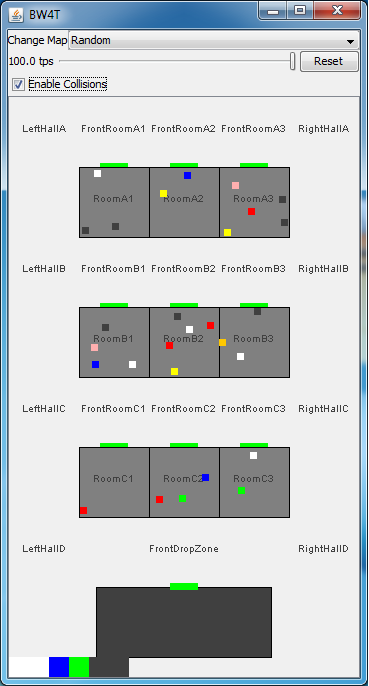
\includegraphics[width=0.48\textwidth]{server.png}
    \caption{Server window}
\end{figure}

\subsection{Advanced run settings}
The default settings for the server can be changed in the command line of your OS. To change the server ip and/or server port execute the following:\\

java –jar bw4t-server.jar –servip $<$server ip here$>$ (default: localhost) –serverport $<$serverport here$>$ (default: 8000)\\

If you change the serverip and/or serverport, change the client settings correspondingly (see below).
The server will now start using the new values.

\section{Running the client (Human Controlled Bot)}
Before running the client, make sure you have already started the server. Start the client.jar in $<$CLIENT$>$. Figure 2 will show up and the bot is automatically added to the server. You can now control the bot by clicking (left or right) at different spots in the Client.
\begin{wrapfigure}{r}{0.5\textwidth}
  \begin{center}
    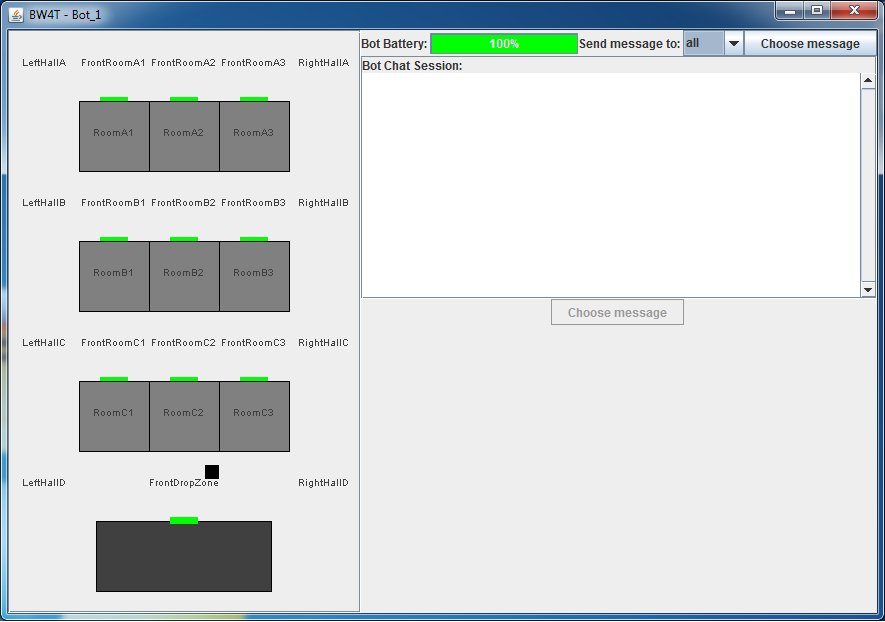
\includegraphics[width=0.6\textwidth]{client.png}
  \end{center}
  \caption{Client window}
\end{wrapfigure}

\section{Running the client (Agent Controlled Bot)}
Before running the client, make sure you have already started the server. Start Eclipse IDE and load your GOAL files. Open the .mas2g file and press the run button. This time, no new window will appear. The agent will control your bot and all evaluations will be shown in the console. In the server window you will see your bot(s) move according to the rules applied in the .goal file(s).

\subsection{Advanced run settings}
The default settings for the client can be changed in the bw4t.mas2g file (GOAL). The following settings can be changed.
\begin{enumerate}
\item Serverip: the ip address that the server listens on (default: localhost).
\item Serverport: the port that the server listens on (default:8000).
\item Agentcount : the amount of agents (also specified in the launchpolicy section, see below), that the client should load. If the agentcount is higher than the amount of entities in the map then they won’t be loaded. (default: 0).
\item Humancount: the amount of human players that should be loaded. If the humancount is higher than the amount of entities in the map then they won’t be loaded. (default: 0).
\item Clientip : the ip address that the client listens on (default: localhost).
\item Clientport : the port that the client listens on (default: 2000).
\item Launchgui: whether to launch a separate GUI for each bot (controlled by an agent or human) can be set to true or false. This GUI shows the environment from the perspective of the bot. (default:false).
\item Map. The map name to be loaded. If you specify a map, the server will reset to load the new map, which disconnects all entities.
\end{enumerate}
The number of agents is specified at two places in the mas2g file. First, the agentcount and humancount specify the number of entities of the corresponding type that should be created in the environment. Second, the launchpolicy specifies which and how many agents should be connected to these entities. Make sure that the agentcount and humancount in the initialization parameters are in line with the launch policy section in the mas2g file. Furthermore, the number of agents should not exceed the maximum number of agents defined on the map (see section “Loading and creating new maps” below).
If you use BW4T from a batch runner, you may want to reset the server after each run. This is done by specifying a map in the mas file init parameters.

\section{Restarting, pausing and resuming the system}
To be able to pause the system, don’t run the mas2g file as described above.
This time, open the mas2g file and click on the debug button (the small bug icon).
\begin{wrapfigure}{r}{0.5\textwidth}
  \begin{center}
    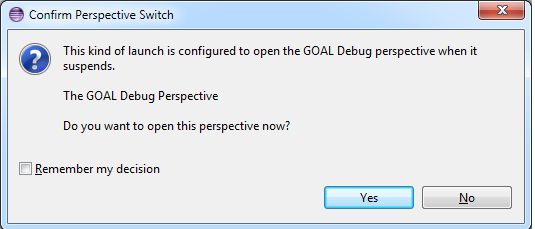
\includegraphics[width=0.6\textwidth]{debug.png}
  \end{center}
  \caption{Choose yes}
\end{wrapfigure}
Eclipse will ask you whether you would like to go to the debug screen (see figure 3), click yes and watch your screen adjust.
Now you can see the running bots listed at the left side, and the current goals, beliefs and knowledge of the selected bot on the right side. Beneath the list the goal file belonging to the bot is shown and at the bottom of the screen, all debug actions are being run. See figure 4.
To pause the system, select the bot to be paused and click on the pause button. To resume, select the bot and click resume.
To restart the system, do the following
\begin{enumerate}
\item In eclipse, kill the MAS by clicking the red box (stop button) at the right of the console window.
\item In the server window, press Reset, or choose a new map from the Change Map menu.
\item Run the MAS in Eclipse as described above.
\end{enumerate}
\begin{figure}
    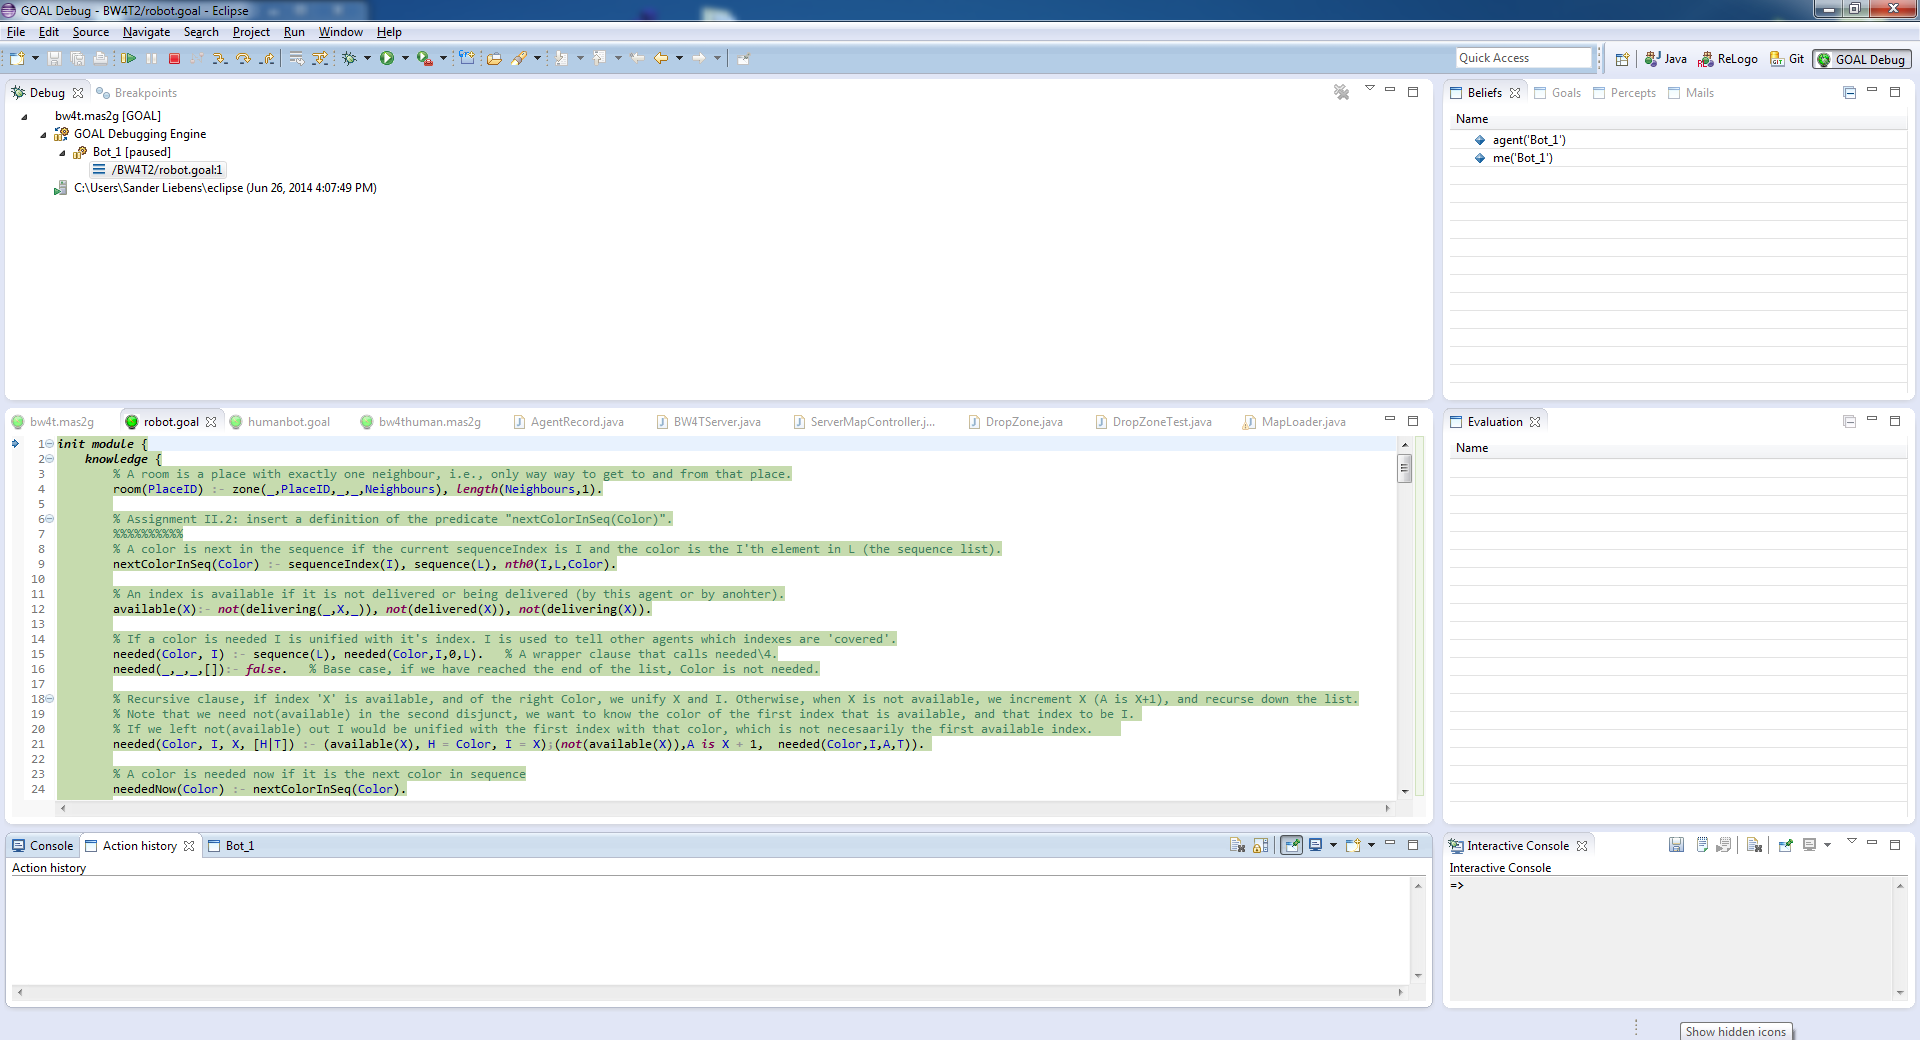
\includegraphics[width=\textwidth]{debugmode.png}
    \caption{Debug mode}
\end{figure}

\newpage
\section{Loading and creating new maps}
\subsection{Using the Environment Store}
The Map Editor is a tool for editing maps for the BW4T server. Double click the jar file environment-store.jar to start the map editor.
\begin{wrapfigure}{r}{0.5\textwidth}
  \begin{center}
    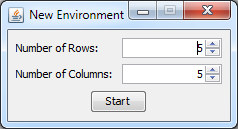
\includegraphics[width=0.6\textwidth]{mapsize.png}
  \end{center}
  \caption{Choose the amount of columns and rows}
\end{wrapfigure}
After starting up, the map size dialog (Figure 5) appears, which can be used as follows.
Here you can choose the amount of rows and columns you want the environment to consist of. Each cell in the “table” can be used to fulfill one piece of the map. This could either be a room, a corridor, a dropzone, a charging zone, start zone or a blockade. By pressing the colours at the bottom you can generate the sequence to be completed. This can also be done by pressing the according numbers on the keyboard. \\
In the Map editor GUI above you can add blocks to rooms. To add blocks to rooms, right click in the cell, adjust the type of the zone to Room. Now you can add blocks the way you did with the sequence. Right clicking the cell again lets you choose at which side of the room you want the door. When you're done, press save. 
By pressing Tools in the menu bar, you are able to randomize zones, blocks and sequences. WARNING: Randomizing these will not always guarantee that the sequence can be completed.
By pressing File in the menu bar, you are able to watch a preview of your map, and you are able to save the map. Save the map in the $<$SERVER$>/$maps folder.
\begin{figure}
    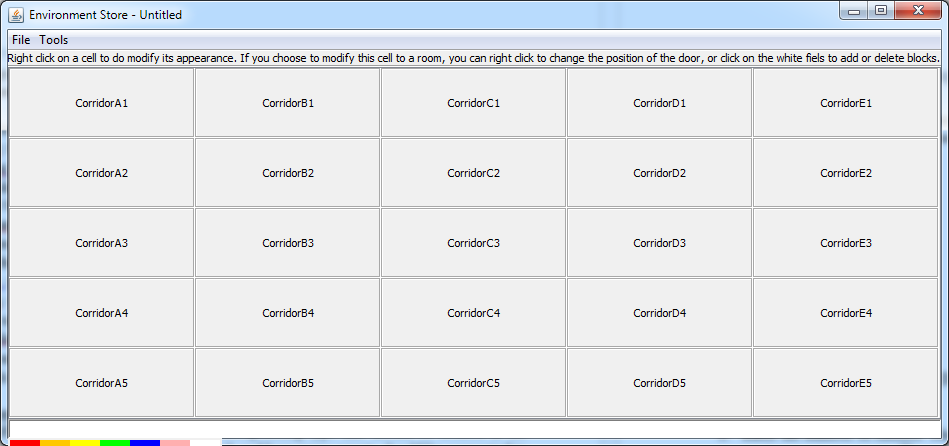
\includegraphics[width=\textwidth]{grid.png}
    \caption{Create a map}
\end{figure}

\newpage
\subsection{Manual editing}
It is also possible to manually edit a map as it is a plain text XML file.
\begin{enumerate}
\item Copy an existing map file in the $<$SERVER$>/$maps folder to a new file.
\item Open the copied map with a text editor. You can then edit the colors in the rooms. Each $<$blocks$>$COL$</$blocks$>$ line inside a $<$zones$>$ of type ROOM adds another block to the room. The currently available colors are BLUE, ORANGE, RED, WHITE, GREEN, YELLOW AND PINK. A room has place for at most 10 blocks.
\item You can change the number of rooms by adding or removing $<$zones$>$ of type ROOM and position the rooms correctly on the map by editing the $<$x$>$ $<$y$>$ $<$width$>$ and $<$height$>$ inside the room's $<$boundingbox$>$. Also you need to add a $<$door$>$ properly positioned on the border of the room.
\item You can edit the goal sequence by adding $<$sequence$>$ items to the map, with colors as mentioned above.
\item You can prevent multiple entities to enter corridor zones by putting true in the item $<$oneBotPerCorridorZone$>$ in the map.
\item You can add entities to the environment by creating more $<$entities$>$ items. Make sure they have a unique $<$name$>$ and that their start position is in a different $<$zone$>$ if you have $<$oneBotPerCorrridorZone$>$ set to true.
\item You can let the server pick a random sequence of a given length by setting the $<$randomSequence$>$ to a positive value. These random blocks are added to the existing sequence items and the random blocks are placed randomly on the map.
\item You can let the server pick random extra blocks to be placed in the rooms on the map by putting a positive number in the $<$randomBlocks$>$ in the map. Note that this addition is on top of all blocks that are already placed in the map; so normally you leave the room zones empty when using this option.
\item You can set per-zone visibility of the zone namelabel in the server map renderer, using a $<$renderOptions$>$ $<$labelVisible$>$ false $</$labelVisible$>$ $</$renderOptions$>$ block to disable visibility.
\item Save the map in the $<$SERVER$>/$maps directory.
\item Edit the map initialization parameter for the server to your new map file. See the section on customizing the server settings. If you now start the server and your new map should be loaded.
\end{enumerate}

\section{Using the interface}
To use the interface, the user clicks with the left (occasionally the right) mouse button in the GUI. Depending on where the user clicks, different menus appear. The user then picks the appropriate action from the menu to execute that action. Below the possibilities are explained.
\subsection{Sending messages}
By clicking on the dropdown menu, the user can choose to which bot he or she will send a request or question. “all” sends the message to all bots. Next to the dropdown menu, a button is placed with choose message. This button contains the messages that are most likely to be sent. Left clicking this button will create a list from which the user can choose a message. When clicking in the “Bot Chat Session”, gives a number of standard answers: yes, no, don't know, ok, etc. It is not possible to use free text because the non-human agents can only process these pre-specified messages. The specification document gives more details on how messages are processed by non-human agents.
\subsection{Click on room or dropzone}
By clicking on a room, the user can order his bot to go to that room, tell everybody something about that room or ask something about that room.
\subsection{Click on blocks}
By clicking on a block (particularly, those below the drop zone), the user can tell everybody something about that block, or ask others for information about that block.
\subsection{Click on hallway}
By clicking on a hallway, the user can point to an exact (X,Y) location to go to. Also it is possible to tell all others roughly where one is in the hallway.

\section{Running on multiple computers}
If you want to run BW4T on multiple computers you should designate one of these computer as the server. On this computer you can start the server as described in the first section of this guide. You must use RMI messaging (check the GOAL Run menu) to allow other GOAL runtimes to connect .
You need to check a few things in the MAS that you use here:
\begin{itemize}
\item specify a map such that the environment resets when you start up the MAS
\item make sure that the map that is used has enough entities to accommodate all agents in all computers that want to connect
\item make sure that the entities get the proper type, by specifying the proper agentcount and humancount.
\end{itemize}
The other computers will then function as client. Create a MAS file for each of these, and configure this MAS as follows (see also bw4thuman.mas2g in the GOALagents directory of GOAL):
\begin{itemize}
\item set the serverip and serverport initialization parameters to the ones that the server is listening on (default for the server is localhost and port 8000).
\item Set the humancount and agentcount parameter on each client to reflect how many human or agent players that client should load.
\item Use humanbot.goal for human agents
\item use env = $<$CLIENT$>/$client.jar". in the environment section. Do not connect to an already running environment in another MAS. This is because BW4TClient creates GUIs for humanbots, on the machine where it is running.
\item Check that the launchpolicy picks up the proper entity type, so use 'human' if you want to attach to human entities etc.
\end{itemize} 

\subsection{Distributed human GUIs}
This section describes how to run a set of distributed human GUIs such that they all communicate through GOAL. Before running a set of distributed Human GUIs with Eclipse, make sure that the server is installed on one machine. Furthermore, make sure that the server map can contain a sufficient number of entities.
To run a set of distributed Human GUIs with GOAL, do the following:
\begin{itemize}
\item Start the server
\item For each machine where you want to have a human GUI:
    \begin{enumerate}
    \item Start  Eclipse IDE
    \item Open the MAS file of the bw4thuman.mas2g
    \item adjust the serverip to correctly point to the machine ip number where the server runs
    \item Start the MAS
    \end{enumerate}
\end{itemize}

\section{Programming a BW4T Agent}
To program your own BW4T agent, use the same actions as specified in the demorobot. You can  choose to change the pre- and post conditions of each action.

Percepts are retrieved automatically by GOAL, see the percept specifications for what percepts you can expect.

In order for messages received by other GOAL agents to appear on the GUI of your agent, you should add the following lines to your GOAL agent’s code:
\begin{enumerate}
\item Add the following line to your knowledge base:\\
\#import “messageTranslation”.
\item Add the following line at the end of your goal file. \\
\#import “message.mod2g”.
\item Add the following line to the start of your event module: \\
if bel(true) then message. \\
This will make sure that the message module that was just imported will be run first when entering the event module.
\item Your own message handling code should be performed after this line and should delete any messages after handling them. Otherwise they will be continuously posted to the GUI as they are not deleted by the message module. If you don’t do any message handling yet you can add the following line below the one provided in step 3 to delete all received messages: \\
forall bel(received(Agt,Msg)) do delete(received(Agt,Msg)).
\end{enumerate}

\subsection{Testing your agent}
In order to test your agent you should edit the bw4t.mas2g file as follows.
\begin{itemize}
\item Add your agent to the agentfiles list.
\item Add a line to the launchpolicy (copy the line of the demorobot and replace 'demorobot' with the name of your agent).
\end{itemize}
Make sure that you set GOAL to launch the desired number of your agent. Also make sure that the initialization parameter of agentcount is not set to 0 as then only humanbots will be loaded.

Note that besides in the bw4t.mas2g file, the number of agents is also specified in the map that you use. This number determines the maximum amount of bots that can appear on the map. If the maximum number of agents to be launched as specified in the bw4t.mas2g file is bigger than the number of agents specified in the map, some of the agents will not appear on the map and not be part of the team. 

\section{Creating your own Scenario}
This part describes how to make use of the Scenario Editor (Figure 7). When you open the editor, you see two main parts:
\begin{enumerate}
\item The Configuration panel, which is used to create, open and save configuration files.
\item The Entity panel, where a list of bots and a list of e-partners are being displayed. Here you can create, modify, rename and delete bots and e-partners.
\end{enumerate}

\begin{figure}[h]
\begin{center}
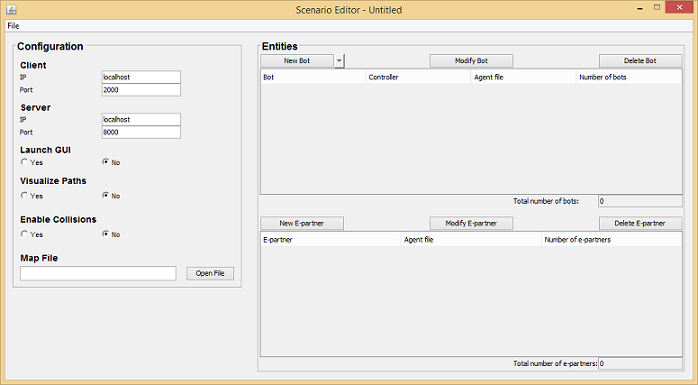
\includegraphics[width=\textwidth]{editor.png}
\caption{Scenario Editor}
\end{center}
\end{figure}

\subsection{General use}
At the top of the editor you can see a $File$ menu. If you click on that, you get the options to create a new configuration,open a configuration, save your configuration, export your configuration and to exit the editor.

On the left side of the editor you can configure a scenario as you like. The Client IP, the Client Port, the Server IP and the Server Port should already contain the default values. You can change them if you need to. You can also indicate whether you want to open a GUI, visualise the paths the bots take or enable collisions. If you have a map file you want to use, you can import it by selecting the $Open$ $file$ button at the right section.

On the right side of the editor you can create, modify, rename and delete bots and e-partners. There also are a list of bots and a list of e-partners that are created, and below each list there is an indication of how many bots or e-partners are created in total.

Linked to the Scenario Editor are the Bot Store and the E-partner Store, which will also be discussed in this document.
\pagebreak
\subsection{Configuration Panel}
A picture of the configuration panel can be found in figure 8.
\begin{figure}[h]
\begin{center}
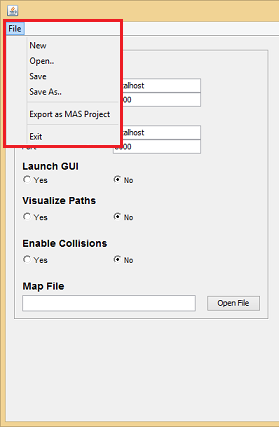
\includegraphics{config.png}
\end{center}
\caption{Configuration Panel}
\end{figure}
\subsubsection{New configuration file}
To create a new configuration file, select $File$ $\to$ $New$ in the menu bar. You will now get a new configuration with the default values. Creating a new configuration will reset all previous changes you have made, so make sure you save your current configuration first if you want to keep it.

\subsection{Open configuration file}
To open an existing configuration file, select $File$ $\to$ $Open$ in the menu bar. A window will pop up where you can select the folder where the configuration file is saved to. Once you have selected the right folder, select the file and click the $Open$ button.

\subsubsection{Save configuration file}
To save your configuration file, select $File$ $\to$ $Save$ in the menu bar. If your file hasn't been saved before, a window will pop up where you can select the folder you want to save your configuration file to and enter the file name you want to use. Once you have selected the right folder and entered the file name, click the $Save$ button.

\subsubsection{Save configuration file as}
To save your configuration in a new file, select $File$ $\to$ $Save$ $As$ in the menu bar. A window will pop up where you can select the folder you want to save your configuration file to and enter the file name you want to use. Once you have selected the right folder and entered the file name, click the $Save$ button.

\subsubsection{Export configuration to mas2g}
To export your configuration to mas2g, you have to have saved your configuration first. Once you have done that, select $File$ $\to$ $Export$ $as$ $MAS$ $project$ in the menu bar. A window will pop up where you can select the folder you want to export the configuration to and the file name you want to use. Once you have selected the right folder and entered the file name, click the $Export$ $MAS$ $project$ button.

\subsubsection{Exit the Scenario Editor}
If you want to close the Scenario Editor, select $File$ $\to$ $Exit$ in the menu bar. Closing the Scenario Editor will not save any changes you have made, so make sure you save your configuration first if you want to keep it.

\subsection{Entity Panel}
The entity panel exists of 2 parts; the top part shows the bot options and the bottom part shows the e-partner options. A picture of the entity panel can be found in figure 9.
\begin{figure}[h]
\begin{center}
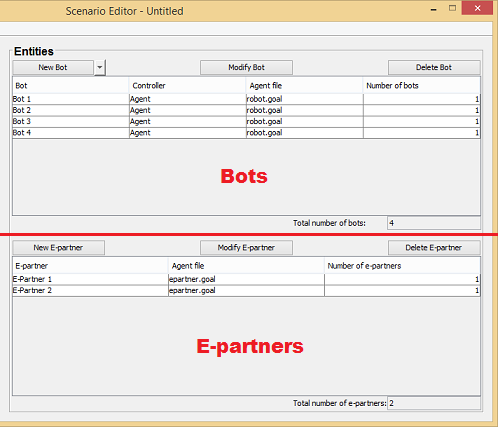
\includegraphics{bot.png}
\end{center}
\caption{Entity Panel}
\end{figure}
\subsubsection{Create new bot}
To create a new bot, click the $New$ $Bot$ button. A new bot will appear in the bot list.\\
If you want to create a standard bot (which already has default values), click on the arrow next to the $New$ $Bot$ button. A menu will drop down where you can select one of the standard bots. If you click on one of the standard bots, the bot will appear in the bot list.

\subsubsection{Modify bot}
To modify a bot, select the bot you want to modify in the bot list and click the $Modify$ $Bot$ button. The Bot Store will open in a new window where you can modify the properties of the bot.

\subsubsection{Rename bot}
To rename a bot, you can either use the $Modify$ $Bot$ button to rename in the Bot Store, or you can rename in the Scenario Editor. To rename in the Scenario Editor, select the bot you want to rename in the list with bots. Double click the its name and enter a new name.

\subsubsection{Change controller type}
To change how a bot is controlled, you can either use the $Modify$ $Bot$ button to change it in the Bot Store, or you can change it in the Scenario Editor. To change the controller type in the Scenario Editor, select the bot you want to change and click on its controller type. You should now be able to choose the controller type.

\subsubsection{Change the amount of entities of a bot}
To change how many entities of a type of bot you want, you can either use the $Modify$ $Bot$ button to change it in the Bot Store, or you can change it in the Scenario Editor. To change the entity amount in the Scenario Editor, select the bot that you want to change the amount of. Now double click the amount given, and enter a new number.

\subsubsection{Delete bot}
To delete a bot, select the bot you want to delete in the list with bots and click the $Delete$ $Bot$ button.

\subsubsection{Create new e-partner}
To create a new e-partner, click the $New$ $E$-$partner$ button. A new e-partner will appear in the e-partner list.

\subsubsection{Modify e-partner}
To modify an e-partner, select the e-partner you want to modify in the e-partner list and click the $Modify$ $E$-$partner$ button. The E-partner Store will open in a new window where you can modify the properties of the e-partner.

\subsubsection{Rename e-partner}
To rename an e-partner, you can either use the $Modify$ $E-partner$ button to rename in the E-partner Store, or you can rename in the Scenario Editor. To rename in the Scenario Editor, select the e-partner you want to rename in the list with e-partners. Double click its name and enter a new name.

\subsubsection{Change the amount of entities of an e-partner}
To change how many entities of a type of e-partner you want, you can either use the $Modify$ $E-partner$ button to change it in the E-partner Store, or you can change it in the Scenario Editor. To change the amount in the Scenario Editor, select the e-partner that you want to change the amount of. Now double click the amount given, and enter a new number.

\subsubsection{Delete e-partner}
To delete an e-partner, select the e-partner you want to delete in the e-partner list and click the $Delete$ $E$-$partner$ button.

\subsection{Bot Store}
A picture of the Bot Store can be found in figure 10.
\begin{figure}[h]
\begin{center}
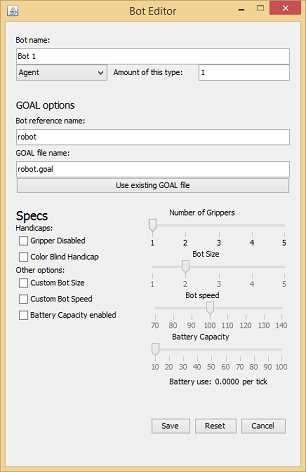
\includegraphics{bs.png}
\end{center}
\caption{Bot Store}
\end{figure}
\subsubsection{Rename bot}
To rename a bot, click on the field that contains its current name. Now you are able to edit the current name or you can enter a new name.

\subsubsection{Change controller type}
To change how a bot is controller, you can click on its current controller type. Now you are able to choose the controller type.

\subsubsection{Change the amount of entities}
To change how many entities of the bot you want, you can click on the field that contains the current number of entities. Now you are able to edit the amount.

\subsubsection{GOAL options}
You can enter the GOAL options for your bot under the $GOAL$ $options$ section. Here you can indicate what its reference name in GOAL should be, and you can select a GOAL agent file which will control the bot. To select the GOAL agent file, you can click on the $Use$ $existing$ $GOAL$ $file$ button. A window will pop up where you can select the folder where the GOAL file is saved to. Once you have selected the right folder, select the file and click the $Open$ button.

\subsubsection{Bot properties}
You can find the available bot properties under the $Properties$ section. To change what properties you want the e-partner to have, you can select or deselect the checkbox next to the property description. Once you have enabled a property, you can use the sliders to change the value of that property.

\subsubsection{Save modifications}
If you want to save the changes you have made to the bot, you can click on the $Save$ button. The Bot Store window will close, and your changes will have been saved.

\subsubsection{Reset modifications}
If you want to reset the changes you have made to the bot, you can click on the $Reset$ button. Your changes will have been reverted to the last saved configuration.

\subsubsection{Cancel modifications}
If you want to cancel modifying the bot without saving any changes, you can click on the $Cancel$ button. The Bot Store window will close.

\subsection{E-partner Store}
A picture of the E-partner Store can be found in figure 11.
\begin{figure}[h]
\begin{center}
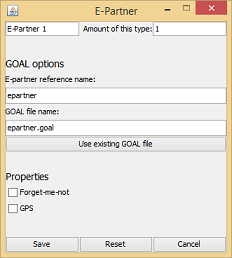
\includegraphics{es.png}
\end{center}
\caption{E-partner Store}
\end{figure}
\subsubsection{Rename e-partner}
To rename an e-partner, click on the field that contains its current name. Now you are able to edit the current name or you can enter a new name.

\subsubsection{Change the amount of entities}
To change how many entities of the e-partner you want, you can click on the field that contains the current number of entities. Now you are able to edit the amount.

\subsubsection{GOAL options}
You can enter the GOAL options for your e-partner under the $GOAL$ $options$ section. Here you can indicate what its reference name in GOAL should be, and you can select a GOAL agent file which will control the e-partner. To select the GOAL agent file, you can click on the $Use$ $existing$ $GOAL$ $file$ button. A window will pop up where you can select the folder where the GOAL file is saved to. Once you have selected the right folder, select the file and click the $Open$ button.

\subsubsection{E-partner properties}
You can find the available e-partner properties under the $Properties$ section. To change what properties you want the e-partner to have, you can select or deselect the checkbox next to the property description.

\subsubsection{Save modifications}
If you want to save the changes you have made to the e-partner, you can click on the $Save$ button. The E-partner Store window will close, and your changes will have been saved.

\subsubsection{Reset modifications}
If you want to reset the changes you have made to the e-partner, you can click on the $Reset$ button. Your changes will have been reverted to the last saved configuration.

\subsubsection{Cancel modifications}
If you want to cancel modifying the e-partner without saving any changes, you can click on the $Cancel$ button. The E-partner Store window will close.

\section{Log file}
Repast logs the following for each run into a file. The filename is “BW4TXXXX.log” where XXX is the date and time to make the filename unique. The file is saved in the $<$SERVER$>/$log directory. It contains:
\begin{enumerate}
\item sequence: goal sequence (which block colors are to be dropped)
\item room: initial blocks per room
\item action: log of each action of a bot, with timestamp 
\item total time: total time to complete task. Begin time is determined by first incoming action. End time is determined by the last block of the sequence dropped.
\item agentsummary: for each agent:
    \begin{itemize}
    \item the bot type containing its handicaps
    \item \# correct drops in dropzone
    \item \# incorrect drops in dropzone
    \item total time of standing still
    \item \# messages to other agents
    \item \# rooms entered
    \end{itemize}
\end{enumerate}
Logs are written to the file as soon as possible, so that information won't get lost when the system is being killed before the end of the sequence is reached.

\end{document}
